%%%%%%%%%%%%%%%%%%%%%%%%%%%%%%%%%%%%%%%%%%%%%%%%%%%%%%%%%%%%%%%%%%%%%%%%
%
%
%     This file is included from the file   Segmentation.tex
% 
%     Section tag and label are placed in this top file.
%
%
%
%%%%%%%%%%%%%%%%%%%%%%%%%%%%%%%%%%%%%%%%%%%%%%%%%%%%%%%%%%%%%%%%%%%%%%%%

\subsection{Introduction}
\label{sec:HybridSegmentationIntroduction}


It is sometimes convenient to combine several segmentation strategies with the
aim of taking advantage of their qualities an compensate their vulnerabilities.
The synergy between fundamentally different methodologies tends to result in
robustness and higher segmentation quality.  This section illustrates an hybrid
approach for segmentation in which two different strategies are configured to
work together. In this case, an input image is first processed by a filter
based on the concept of region growing. The criterion of acceptance in the
region is defined by a similarity measure that evaluates how homogeneous is the
path between to pixels. The output of this filter is used as a prior for
another filter that performs a full partition of the image space and then work
joining and splitting regions in order to optimize an homogeneity measure.
Details on the concepts behind those methods have been discussed in the
litterature
\cite{Angelini2002,Udupa2002,Jin2002,Imielinska2001,Imielinska2000a,Imielinska2000b}



\subsection{Background}
\label{sec:HybridSegmentationBackground}




%%%%%%%%%%%%%%%%%%%%%%%%%%%%%%%%%%%%%%%%%%%%%%%%%%%%%%%%%%%%%%%%%
%
%  Here is an example of how to include diagram in a figure
%
%  The file HybridSegmentationDiagram1.fig should be in the "Art"
%  directory. CMake will convert it to EPS before running latex. 
%
%%%%%%%%%%%%%%%%%%%%%%%%%%%%%%%%%%%%%%%%%%%%%%%%%%%%%%%%%%%%%%%%%

\begin{figure}
\center
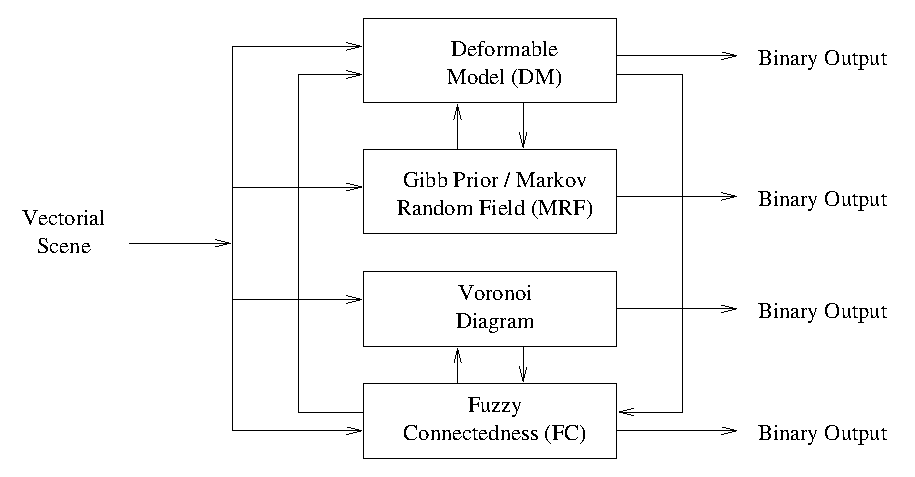
\includegraphics[width=6cm]{HybridSegmentationEngine1.eps}
\caption{Components of a HybridSegmentation approach}
\label{fig:HybridSegmentationEngine1}
\end{figure}

The Figure \ref{fig:HybridSegmentationEngine1} illustrates the main
components of the hybrid segmentation algorithm.

\begin{figure}
\center
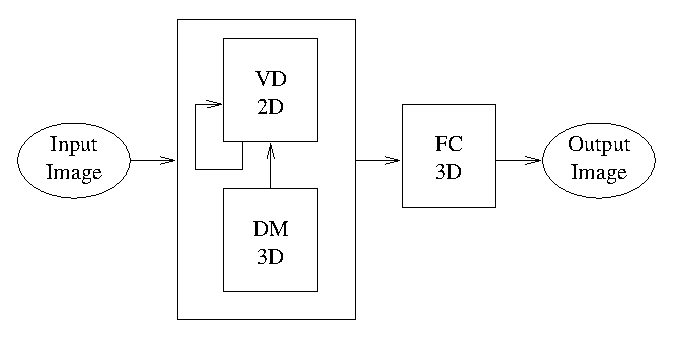
\includegraphics[width=6cm]{HybridSegmentationFCVDDM.eps}
\caption{Components of a HybridSegmentation approach}
\label{fig:HybridSegmentationFCVDDM}
\end{figure}


\begin{figure}
\center
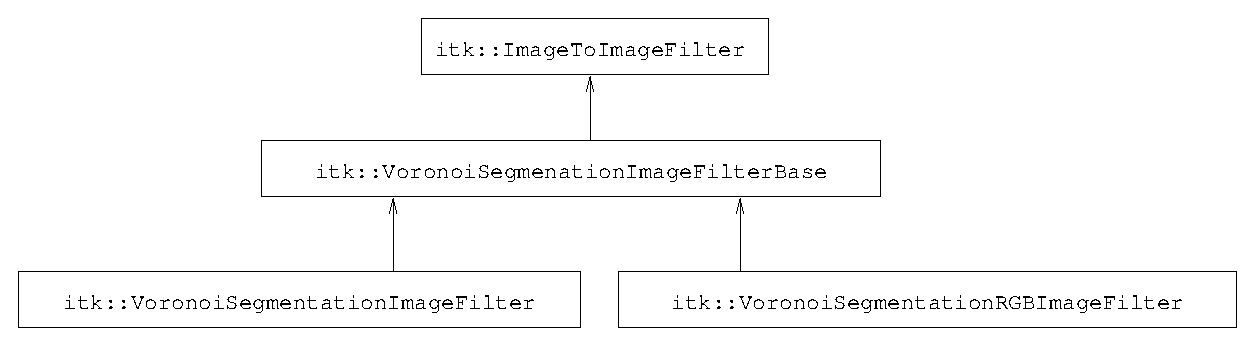
\includegraphics[width=6cm]{VoronoiSegmentationClassDiagram1.eps}
\caption{UML Class Diagram of the VoronoiSegmentation filter}
\label{fig:VoronoiSegmentationClassDiagram1}
\end{figure}


\begin{figure}
\center
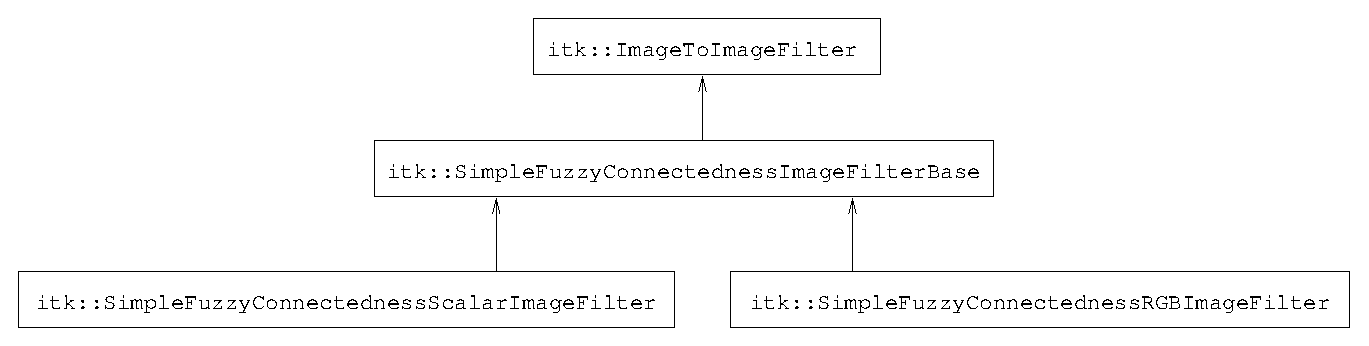
\includegraphics[width=6cm]{FuzzyConnectednessClassDiagram1.eps}
\caption{UML Class Diagram of the FuzzyConnectedness filter}
\label{fig:FuzzyConnectednessClassDiagram1}
\end{figure}


\begin{figure}
\center
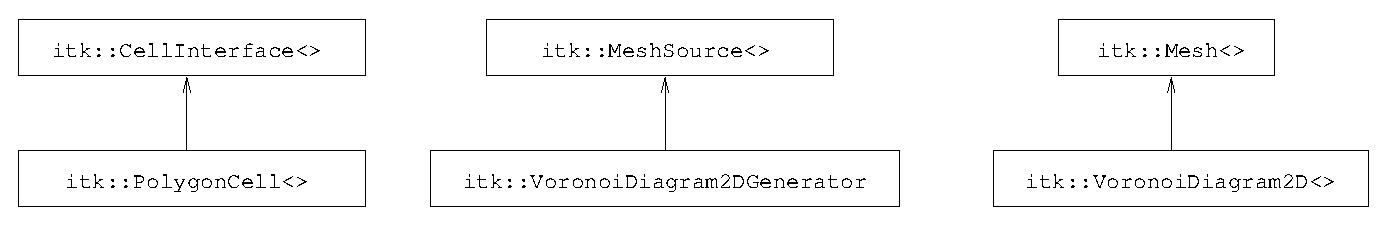
\includegraphics[width=6cm]{VoronoiSegmentationCollaborationDiagram1.eps}
\caption{UML Collaboration Diagram of the VoronoiSegmentation filter}
\label{fig:VoronoiSegmentationCollaborationDiagram1}
\end{figure}



\begin{figure}
\center
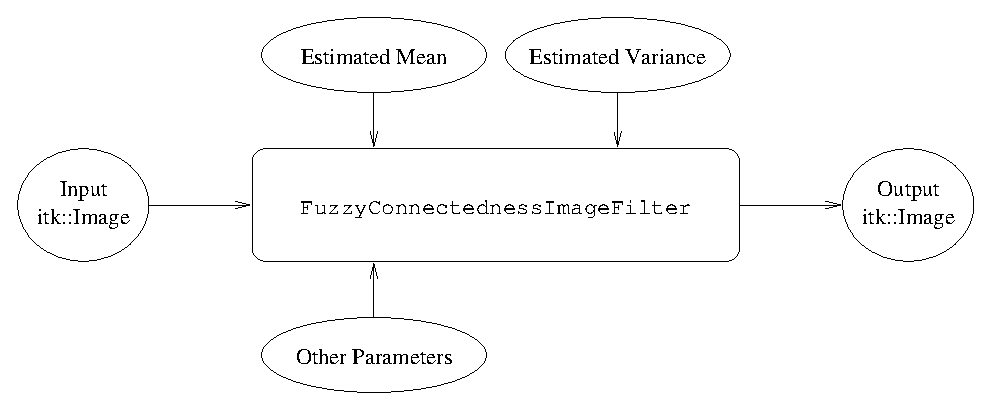
\includegraphics[width=6cm]{FuzzyConnectednessCollaborationDiagram1.eps}
\caption{UML Collaboration Diagram of the FuzzyConnectedness filter}
\label{fig:FuzzyConnectednessCollaborationDiagram1}
\end{figure}



\begin{figure}
\center
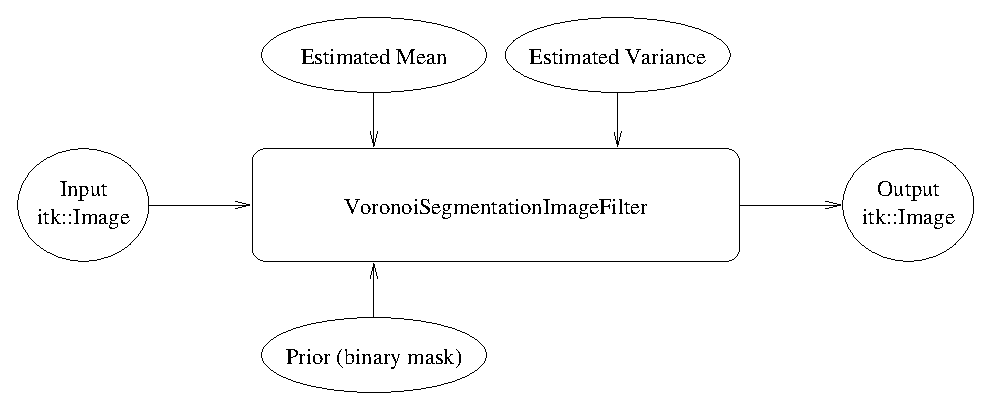
\includegraphics[width=6cm]{VoronoiSegmentationCollaborationDiagram2.eps}
\caption{UML Collaboration Diagram of the VoronoiSegmentation filter}
\label{fig:VoronoiSegmentationCollaborationDiagram2}
\end{figure}




\begin{figure}
\center
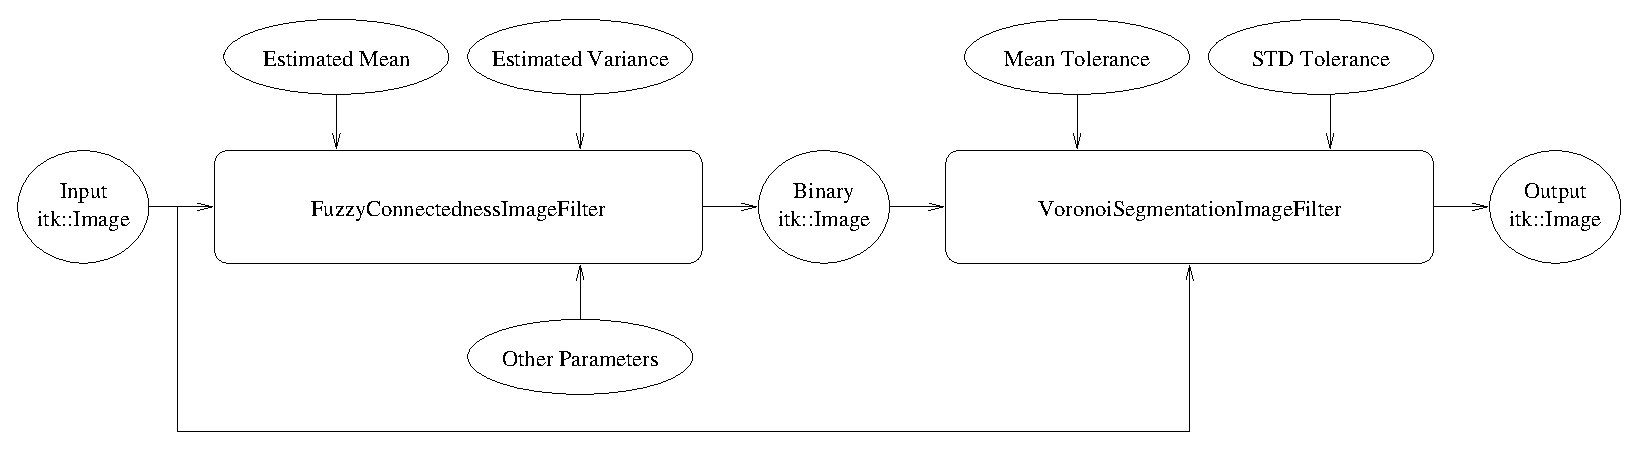
\includegraphics[width=6cm]{FuzzyVoronoiCollaborationDiagram1.eps}
\caption{UML Collaboration Diagram of the Fuzzy Voronoi Segmentation}
\label{fig:FuzzyVoronoiCollaborationDiagram1}
\end{figure}




\begin{figure}
\center
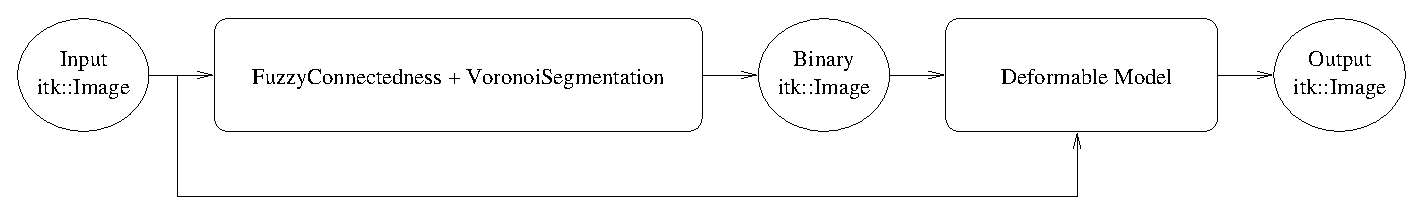
\includegraphics[width=6cm]{FuzzyVoronoiDeformableCollaborationDiagram1.eps}
\caption{UML Collaboration Diagram of the Fuzzy Voronoi Deformable Segmentation}
\label{fig:FuzzyVoronoiDeformableCollaborationDiagram1}
\end{figure}









%%%%%%%%%%%%%%%%%%%%%%%%%%%%%%%%%%%%%%%%%%%%%%%%%%%%%%%%%%%%%%%%%
%
%  Here is an example of how to include equations
%
%%%%%%%%%%%%%%%%%%%%%%%%%%%%%%%%%%%%%%%%%%%%%%%%%%%%%%%%%%%%%%%%%


\begin{equation}
MS(A,B) = \frac{1}{N} \sum_i^N \left( A_i - B_i \right)^2
\end{equation}





\subsection{Example}
\label{sec:HybridSegmentationExample1}

\input{HybridSegmentationFuzzyVoronoi.tex}


